When you run \emph{Flat Hunt}, the first you'll see is a menu (see \autoref{settings_screenshot}). You can either let the default options in place and just select \emph{start game} or you can adjust the settings to your needs. \emph{Game mode} is explained in \autoref{game_modes}, \emph{number of hunters} and \emph{map size} should be self-explanatory and \emph{characters} specifies which pictures to use for the players. To toggle between the settings menu and the normal menu press \emph{tab}.\\
\begin{figure}[h]
  \centerline{\hbox{
    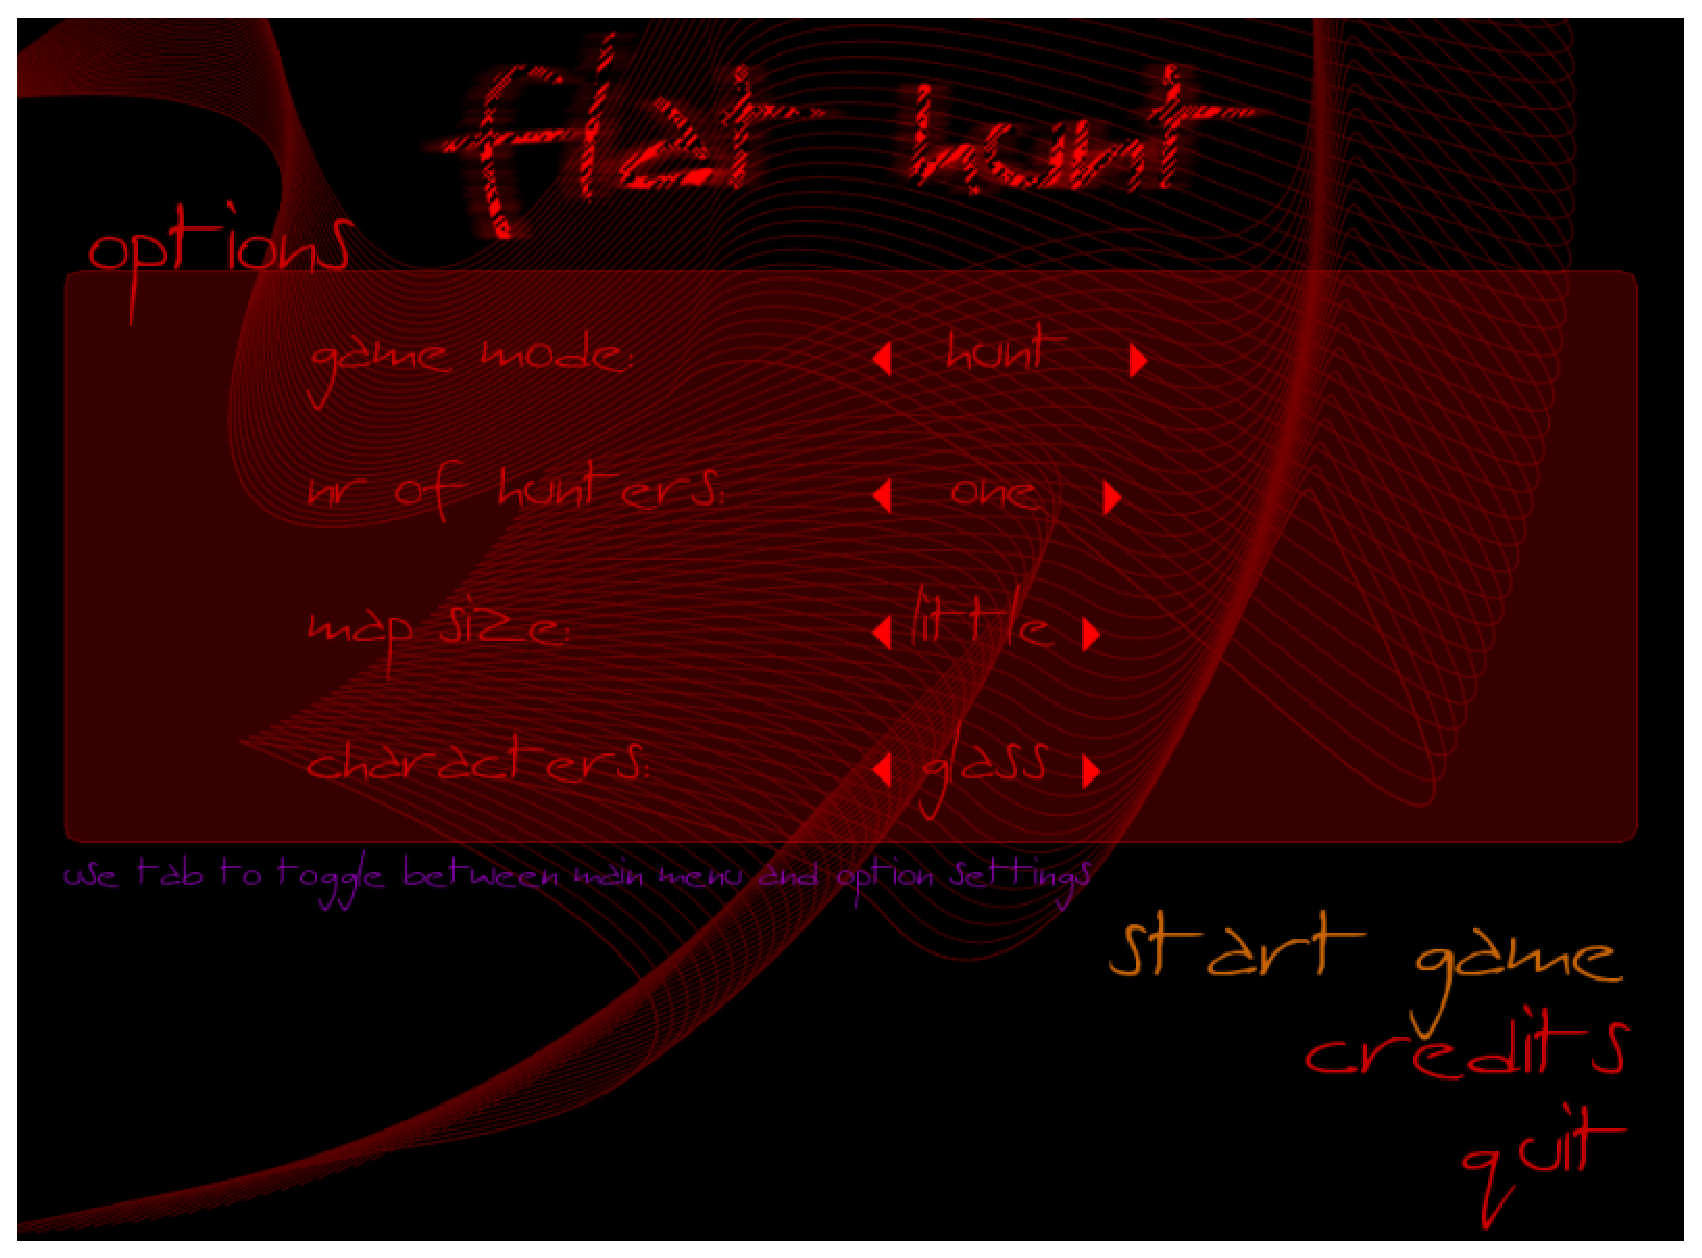
\includegraphics[width=135mm]{settings_screenshot}
  }}
\caption{Screenshot of the start menu}
\label{settings_screenshot}
\end{figure}

  During the game when you press \emph{p}, the pause menu is shown. \emph{Continue} makes the pause menu disappear and lets you resume the game, \emph{new game} takes you to the start menu and \emph{quit} quits the application.\\

  The game over menu is similar to the pause menu, only there is no \emph{continue} in this one.
